\section{Experiments}

\subsection{Machine Learning for Puzzle Complexity Function}

Our method of determining puzzle difficulty was to use machine learning to categorize a puzzle's characterizing vector. To test the reliability of this approach, we recorded published puzzles and their respective difficulty levels from online puzzle providers. This database of puzzles was randomly divided into two sets: a training set and a testing set. The training set was used to generate the SVM's categorization function, and the testing set was used to generate the "success rate": the percentage of puzzles in the testing set whose SVM-determined difficulty matched the difficulty assigned by the puzzle providers. 

$\space$

For our sudoku database, we recorded 206 puzzles from Web Sudoku, the largest online sudoku puzzle provider. For our fillomino database, we recorded 40 puzzles from Math In English, a puzzle website that had categorized puzzles by difficulty levels similar to those of Web Sudoku: (1) Easy, (2) Moderate, (3) Challenging, and (4) Super Difficult. Below are graphs of the average success rates of 500 trials as the percentage of puzzles in the training set was increased.  

$\space$

\centerline{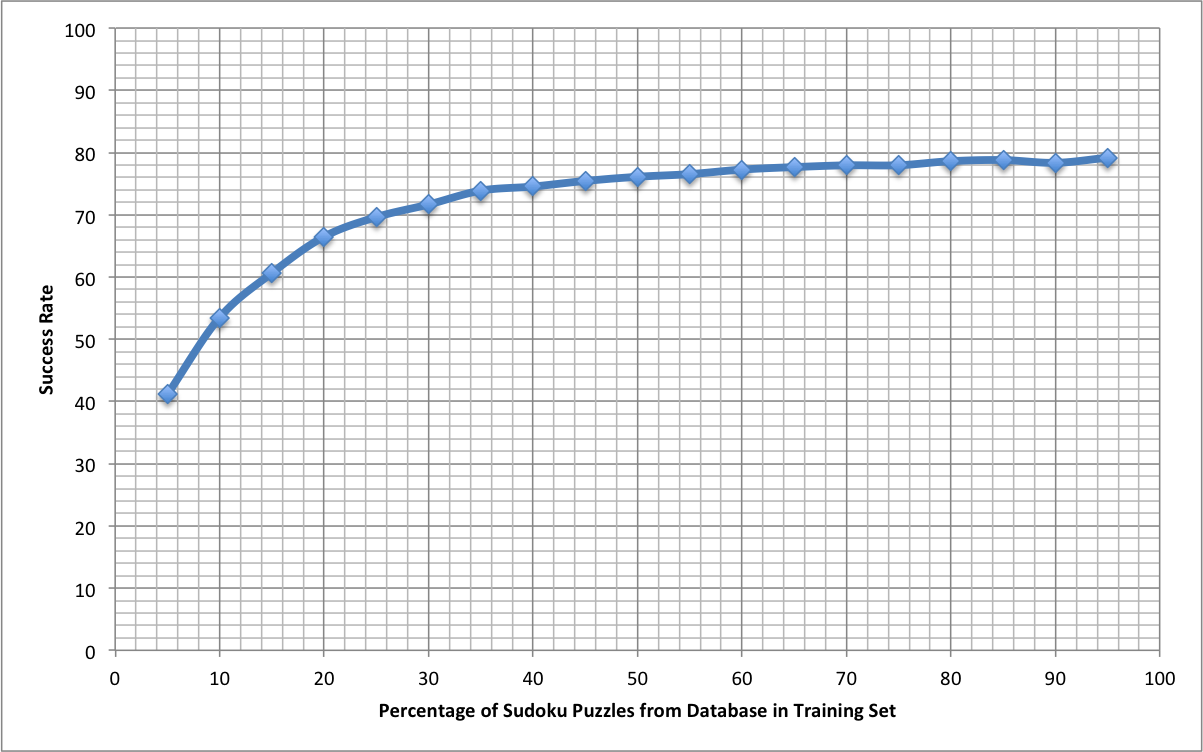
\includegraphics[height = 7cm]{SudokuDifficulty.png}}

$\space$

\centerline{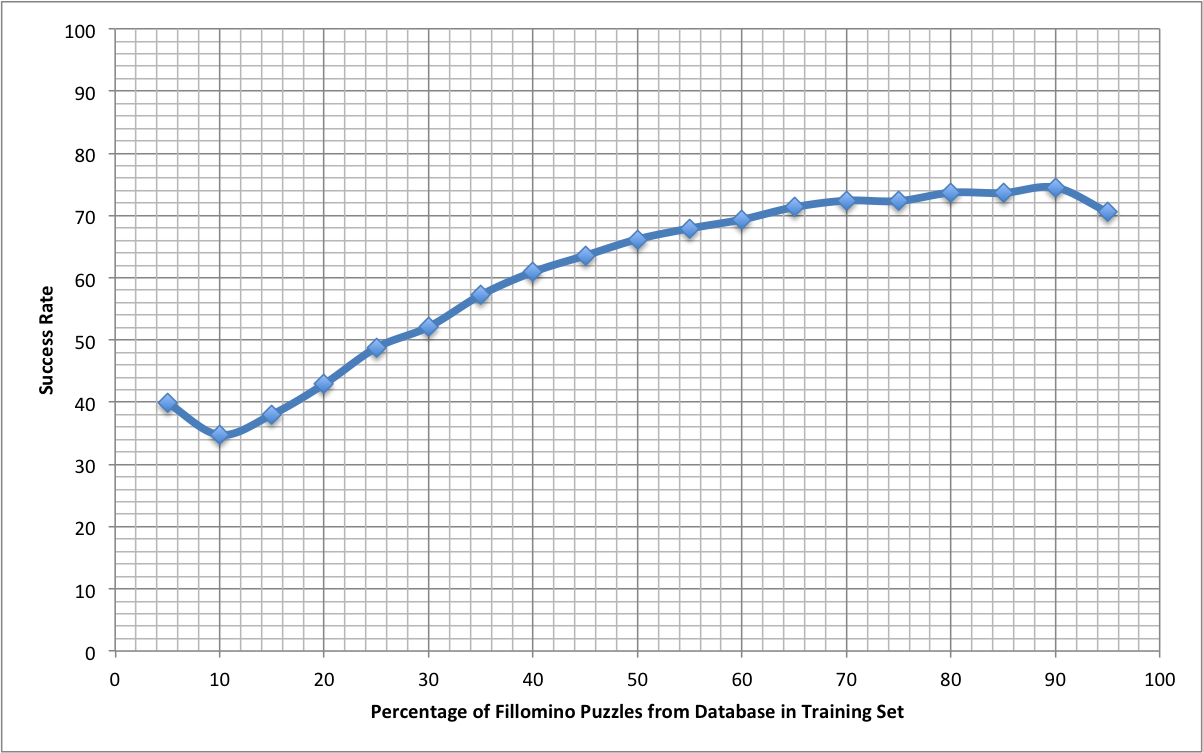
\includegraphics[height = 7cm]{FillominoDifficulty.png}}

$\space$

Our results show that as we increased the number of puzzles in the training set, the success rate increased to $80 \%$.

\subsection{Scalability of Our Approach}

To test the scalability of our puzzle generation algorithm, we generated 16x16 and 25x25 sudoku boards to compare with the standard 9x9 boards and all square fillomino boards from 2x2 to 16x16.

$\space$

When we empty a puzzle with dimensions NxN, we set as a parameter the target number of cells that the program would aim to empty from an initially full board. When the program reaches a point where it cannot further empty any more cells (i.e. the emptying of any remaining cell would cause the board to have more than the maximum number of allowable solutions), the emptying process will be considered finished. Because of this, we observe stagnation in our run times as the target number of empty cells is increased beyond a certain threshold. 

$\space$

The graph below shows program running times to create and empty 9x9, 16x16, and 25x25 Sudoku puzzles as the target number of empty squares is increased. There is an exponential increase in run time as the number of possible empty spaces increased. Even for 25x25 sudoku puzzles, we find that the time required to generate a sudoku puzzle is quite reasonable (around 500 seconds).

$\space$

\centerline{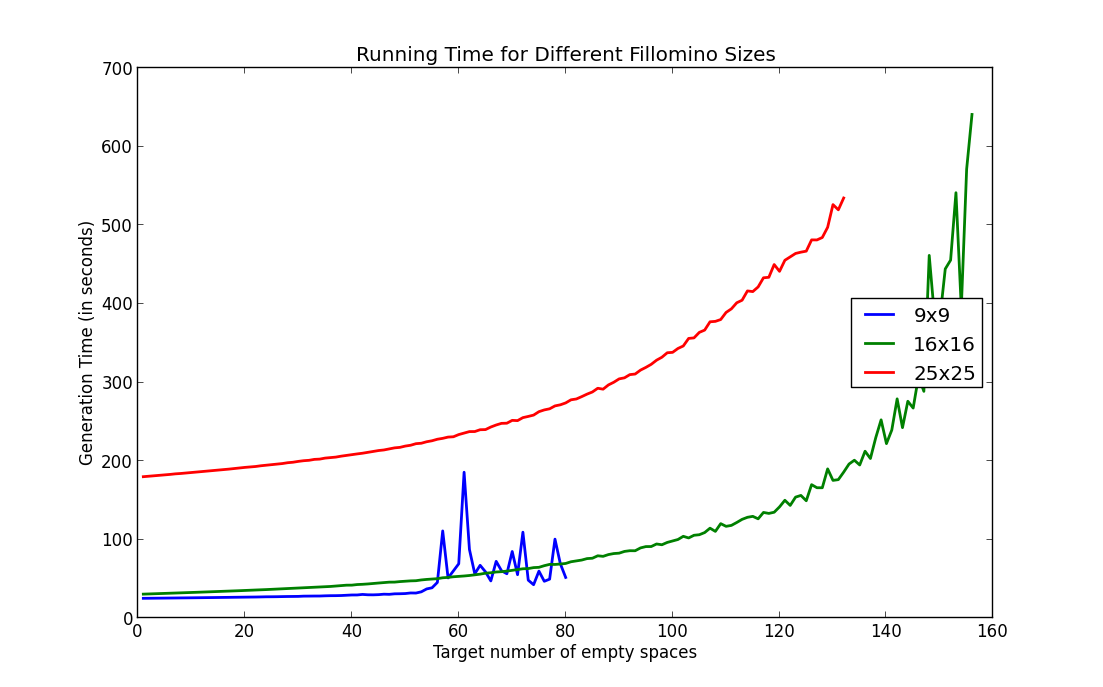
\includegraphics[height = 7cm]{sudoku2.png}}

$\space$


We can see in the graph that the generation time for 9x9 puzzles does not continue to increase after the target number of empty cells was raised beyond 60 because the emptying had stopped before the target of 60+ empty cells had been reached. 

$\space$

A similar experiment with Fillomino puzzles demonstrates a similar pattern of stagnation after a threshold. Unlike the run times of Sudoku puzzles, however, the run times for fillomino puzzles follow a linear trend, not an exponential trend, as the target number of empty spaces is increased.

$\space$

\centerline{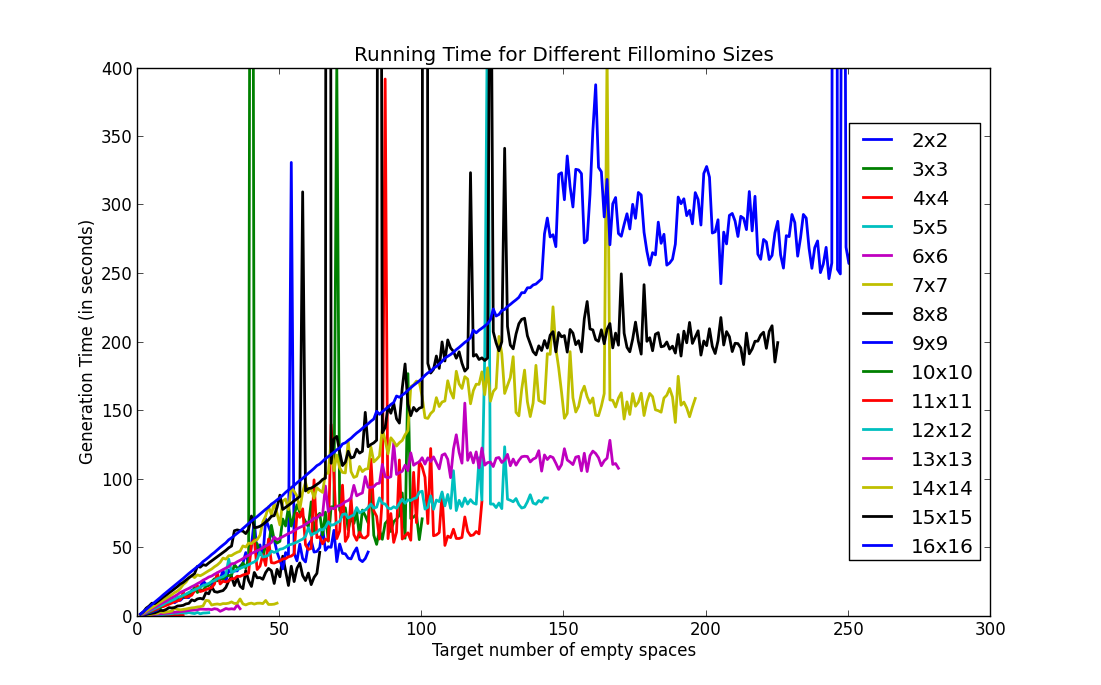
\includegraphics[height = 7cm]{fillomino2.png}}

$\space$





